% config.tex
% 指定 XeLaTeX 编译
%!TeX program = xelatex

%%%%%%%%%%%%%%%%%%%%%%%%%%%%%%%%%%%%%%%%%%%%%%%%%%%%%%%%%%
% 文档类与全局设置
%%%%%%%%%%%%%%%%%%%%%%%%%%%%%%%%%%%%%%%%%%%%%%%%%%%%%%%%%%
\documentclass{beamer}
%tikz包
\usepackage{amsmath, amssymb, xcolor, tikz}
\usetikzlibrary{calc}  % 计算坐标
\usetikzlibrary{backgrounds}  % 背景支持(如果想使用 on background layer)
\usepackage[most]{tcolorbox}
\usepackage{xparse}

% 采用 XeLaTeX 时加载 fontspec 与 xeCJK,实现中西文字体统一管理
\usepackage{fontspec}
\usepackage{xeCJK}
\usepackage{fontspec}
\usepackage{unicode-math}

% 设置英文字体
\setmainfont{Liberation Sans} 
\setsansfont{Liberation Sans}
\setmonofont{Liberation Mono}
% 设置数学公式字体
\setmathfont{TeX Gyre Termes Math} % 数学部分使用 New Roman 风格字体

% 设置中文字体(可根据需求调整)
\usepackage{xeCJK}
\setCJKmainfont{Noto Sans CJK SC} % 主要中文黑体
\setCJKsansfont{Noto Sans CJK SC}
\setCJKmonofont{Noto Sans CJK SC}
% 如果不需要区分宋体或黑体,相关宏定义可以省略

%%%%%%%%%%%%%%%%%%%%%%%%%%%%%%%%%%%%%%%%%%%%%%%%%%%%%%%%%%
% 图形、色彩与数学设置
%%%%%%%%%%%%%%%%%%%%%%%%%%%%%%%%%%%%%%%%%%%%%%%%%%%%%%%%%%
\usepackage{tikz}
\usepackage[table]{xcolor}    % 表格色块
\usepackage{booktabs}         % 三线表格式
\usepackage{pgfplots}
\pgfplotsset{compat=1.18}

\usepackage{tcolorbox}
\usepackage{amsmath}
\usepackage{xcolor}

\usepackage{unicode-math}
\setmathfont{TeX Gyre Termes Math}
\setbeamercolor{block title}{fg=black,bg=gray!10}
\setbeamerfont{block title}{size=\normalsize,family=\rmfamily}


%%%%%%%%%%%%%%%%%%%%%%%%%%%%%%%%%%%%%%%%%%%%%%%%%%%%%%%%%%
% Beamer 主题与风格设置
%%%%%%%%%%%%%%%%%%%%%%%%%%%%%%%%%%%%%%%%%%%%%%%%%%%%%%%%%%
% 清除默认页眉与 frametitle 模板(后续自定义)
\setbeamertemplate{headline}{}
\setbeamertemplate{frametitle}{}
\setbeamertemplate{itemize item}[circle]

% 内外主题(可根据需求替换)
\useoutertheme[subsection=true]{miniframes} 
\useinnertheme{default}
\usecolortheme{default}

%%%%%%%%%%%%%%%%%%%%%%%%%%%%%%%%%%%%%%%%%%%%%%%%%%%%%%%%%%
% 颜色定义(可自定义调色板)
%%%%%%%%%%%%%%%%%%%%%%%%%%%%%%%%%%%%%%%%%%%%%%%%%%%%%%%%%%
\definecolor{lightblue}{RGB}{70,130,180}
\definecolor{midblue}{RGB}{28,70,130}
\definecolor{darkblue}{RGB}{10,40,80}
\definecolor{myred}{RGB}{150,50,30}
\definecolor{mygreen}{RGB}{45,125,77}
\definecolor{mypurple}{RGB}{120,61,137}
\definecolor{myorange}{RGB}{190,88,32}
\definecolor{myitem}{RGB}{35,35,35}


%%%%%%%%%%%%%%%%%%%%%%%%%%%%%%%%%%%%%%%%%%%%%%%%%%%%%%%%%%
% 导航栏与页眉设置
%%%%%%%%%%%%%%%%%%%%%%%%%%%%%%%%%%%%%%%%%%%%%%%%%%%%%%%%%%
% 设置顶部导航栏(用于章节、子章节导航)
\setbeamertemplate{headline}{%
  \begin{beamercolorbox}[wd=\paperwidth,ht=2ex,dp=1ex]{section in head/foot}
    \insertsectionnavigationhorizontal{\paperwidth}{}{}%
  \end{beamercolorbox}%
}
\setbeamercolor{section in head/foot}{bg=darkblue, fg=white}
\setbeamercolor{subsection in head/foot}{bg=midblue, fg=white}

% 自定义非封面页的页眉(显示 frametitle)
\setbeamertemplate{headline}{%
  \ifnum\value{framenumber}>1
    \begin{tikzpicture}[remember picture,overlay]
      % 使用 \raisebox 可微调文本基线,保持与正文垂直居中
      \node[anchor=west, font=\normalsize, text=black, xshift=0.2cm, yshift=-0.4cm]
            at (current page.north west){\insertframetitle};
      \draw[line width=1pt, color=midblue]
            ([yshift=-0.7cm]current page.north west) -- ([yshift=-0.7cm]current page.north east);
    \end{tikzpicture}
  \fi
}

%%%%%%%%%%%%%%%%%%%%%%%%%%%%%%%%%%%%%%%%%%%%%%%%%%%%%%%%%%
% 图注样式设置
%%%%%%%%%%%%%%%%%%%%%%%%%%%%%%%%%%%%%%%%%%%%%%%%%%%%%%%%%%
\setbeamerfont{caption}{size=\footnotesize}
\setbeamercolor{caption}{fg=black}
% 此处使用默认字体,确保中文统一为 Noto Sans CJK SC
\setbeamerfont{caption name}{size=\footnotesize}
\setbeamercolor{caption name}{fg=black}
\setbeamertemplate{caption}[numbered]
\renewcommand{\figurename}{图}

%%%%%%%%%%%%%%%%%%%%%%%%%%%%%%%%%%%%%%%%%%%%%%%%%%%%%%%%%%
% 列表样式设置
%%%%%%%%%%%%%%%%%%%%%%%%%%%%%%%%%%%%%%%%%%%%%%%%%%%%%%%%%%
% 自定义无序列表图标,采用 \raisebox 微调图标位置
\newcommand{\useBigCircleItem}{%
  \setbeamertemplate{itemize item}{\raisebox{0.3ex}{\tikz{\draw[myitem, fill=myitem] (0,0) circle (2pt);}}}%
  \setbeamertemplate{itemize subitem}{\raisebox{0.3ex}{\tikz{\draw[myitem, fill=myitem] (0,0) circle (2pt);}}}%
  \setbeamertemplate{itemize subsubitem}{\raisebox{0.3ex}{\tikz{\draw[myitem, fill=myitem] (0,0) circle (2pt);}}}%
}
\newcommand{\useSmallCircleItem}{%
  \setbeamertemplate{itemize item}{\raisebox{0.35ex}{\tikz{\draw[myitem, fill=myitem, opacity=0.8] (0,0) circle (1pt);}}}%
  \setbeamertemplate{itemize subitem}{\raisebox{0.35ex}{\tikz{\draw[myitem, fill=myitem, opacity=0.8] (0,0) circle (1pt);}}}%
  \setbeamertemplate{itemize subsubitem}{\raisebox{0.35ex}{\tikz{\draw[myitem, fill=myitem, opacity=0.8] (0,0) circle (1pt);}}}%
}
% 默认使用大圆圈
\useBigCircleItem

% 有序列表样式
\setbeamercolor{enumerate item}{fg=darkblue}
\setbeamertemplate{enumerate item}{%
  \usebeamerfont*{enumerate item}%
  \color{enumerate item.fg}\insertenumlabel.%
}

%%%%%%%%%%%%%%%%%%%%%%%%%%%%%%%%%%%%%%%%%%%%%%%%%%%%%%%%%%
% 页脚设置
%%%%%%%%%%%%%%%%%%%%%%%%%%%%%%%%%%%%%%%%%%%%%%%%%%%%%%%%%%
\setbeamertemplate{footline}{%
  \begin{tikzpicture}[remember picture,overlay]
    \node[fill=lightblue, minimum width=0.3\paperwidth, minimum height={0.4cm+1pt}, anchor=south west]
         at ([xshift=-1pt,yshift=-1pt]current page.south west) (leftblock) {};
    \node[fill=midblue, minimum width=0.6\paperwidth, minimum height={0.4cm+1pt}, anchor=south west]
         at ([xshift=0.3\paperwidth-1pt,yshift=-1pt]current page.south west) (midblock) {};
    \node[fill=darkblue, minimum width={0.1\paperwidth+1pt}, minimum height={0.4cm+1pt}, anchor=south west]
         at ([xshift=0.9\paperwidth-1pt,yshift=-1pt]current page.south west) (rightblock) {};
    \node[anchor=center, yshift=0.5pt, font=\tiny, text=white] at (leftblock.center)
         {程明明, http://mmcheng.net};
    \node[anchor=center, yshift=0.5pt, font=\tiny, text=white] at (midblock.center)
         {大规模图像的多粒度目标检测};
    \node[anchor=center, yshift=0.5pt, font=\tiny, text=white] at (rightblock.center)
         {\insertframenumber};
  \end{tikzpicture}
}

%%%%%%%%%%%%%%%%%%%%%%%%%%%%%%%%%%%%%%%%%%%%%%%%%%%%%%%%%%
% 表格样式宏定义
%%%%%%%%%%%%%%%%%%%%%%%%%%%%%%%%%%%%%%%%%%%%%%%%%%%%%%%%%%
\newcommand{\PlainTable}[1]{%
  {\footnotesize
   \setlength{\tabcolsep}{6pt}%
   #1%
  }%
}
\newcommand{\ThreeLineTable}[1]{%
  {\footnotesize
   \setlength{\tabcolsep}{6pt}%
   #1%
  }%
}
\newcommand{\AltColorTable}[1]{%
  {\footnotesize
   \setlength{\tabcolsep}{6pt}%
   \rowcolors{2}{gray!20}{white}%
   #1%
   \rowcolors{2}{}{}%
  }%
}

%%%%%%%%%%%%%%%%%%%%%%%%%%%%%%%%%%%%%%%%%%%%%%%%%%%%%%%%%%
%强调块(适用于公式等)
%%%%%%%%%%%%%%%%%%%%%%%%%%%%%%%%%%%%%%%%%%%%%%%%%%%%%%%%%%
% 定义参数 key 和默认值
\pgfkeys{
  /BehindEqBox/.is family, /BehindEqBox,
  color/.initial = midblue,
  border/.initial = 1pt,
  style/.initial = solid,
  padding/.initial = 2.8mm
}

% 定义命令:支持键值对参数 + 内容
\NewDocumentCommand{\BehindEqBox}{O{} m}{%
  % 加载参数
  \pgfkeys{/BehindEqBox, #1}

  \vspace{1em}
  \begin{center}
    \begin{tikzpicture}[remember picture, overlay]
      \node[inner sep=\pgfkeysvalueof{/BehindEqBox/padding}] (E) {#2};

      \coordinate (A) at ([xshift=-25pt]E.south west);
      \coordinate (B) at ([xshift=25pt]E.north east);

      \begin{pgfonlayer}{background}
        \filldraw[fill=\pgfkeysvalueof{/BehindEqBox/color}, opacity=0.1, rounded corners=0.35cm]
          (A) rectangle (B);

        \draw[
          line width=\pgfkeysvalueof{/BehindEqBox/border},
          draw=\pgfkeysvalueof{/BehindEqBox/color},
          opacity=0.2,
          rounded corners=0.35cm,
          \pgfkeysvalueof{/BehindEqBox/style}
        ] 
        (A) rectangle (B);
      \end{pgfonlayer}
    \end{tikzpicture}
  \end{center}
  \vspace{1em}
}


%%%%%%%%%%%%%%%%%%%%%%%%%%%%%%%%%%%%%%%%%%%%%%%%%%%%%%%%%%
%字体高亮块
%%%%%%%%%%%%%%%%%%%%%%%%%%%%%%%%%%%%%%%%%%%%%%%%%%%%%%%%%%
% 替换原 block 环境
\newtcolorbox{beamerblockbox}[3][]{%
  enhanced,
  breakable,
  colback=#2!10,             % 内容背景(透明度 80%)
  colframe=#2,               % 框颜色 = 标题栏颜色
  coltitle=white,            % 标题文字颜色
  fonttitle=\large,
  title=#3,
  boxed title style={
    colback=#2,
    top=2pt, bottom=2pt,
    left=2pt, right=2pt,
    sharp corners=northwest,
    sharp corners=northeast,
  },
  boxrule=0pt,
  arc=1.5mm,
  shadow={0pt}{-1pt}{1.5mm}{black!30},
  left=2pt, right=2pt,
  top=2pt, bottom=2pt,
  before skip=6pt,  % block与上文之间的空隙
  #1,
}

% 替换默认 beamer block 环境
\let\oldblock\block
\renewenvironment{block}[1]{\begin{beamerblockbox}{midblue}{#1}}{\end{beamerblockbox}}

\let\oldalertblock\alertblock
\renewenvironment{alertblock}[1]{\begin{beamerblockbox}{myred}{#1}}{\end{beamerblockbox}}

\let\oldexampleblock\exampleblock
\renewenvironment{exampleblock}[1]{\begin{beamerblockbox}{myorange}{#1}}{\end{beamerblockbox}} % 导入配置文件
\useSmallCircleItem

\begin{document}

%%%%%%%%%%%%%%%%%%%%%%%%%%%%%%%%%%%%%%%%%%%%%%%%%%%%%%%%%%
%封面页
%%%%%%%%%%%%%%%%%%%%%%%%%%%%%%%%%%%%%%%%%%%%%%%%%%%%%%%%%%
\newcommand{\mytitle}{The title of the presentation is here}
\newcommand{\myauthor}{Your Name}
\newcommand{\myinstitute}{Nankai University}

\begin{frame}
  \begin{tikzpicture}[remember picture, overlay]
    % 蓝色标题栏背景
    \node[fill=midblue, inner sep=0pt, outer sep=0pt, 
      minimum width=\paperwidth, 
      minimum height=0.5\paperheight, 
      anchor=north] at ([yshift=+1pt]current page.north) {};
    
    % 标题
    \node[text=white, 
          font=\fontsize{32}{36}\selectfont\bfseries, 
          text width=0.9\paperwidth, 
          align=center] at ([yshift=-0.265\paperheight]current page.north) 
          {\mytitle};
    
    % 作者信息
    \node[text=black, 
          font=\Large] at ([yshift=-1.5cm]current page.center) 
          {\myauthor};
    
    % 机构信息
    \node[text=black, 
          font=\Large] at ([yshift=-2.5cm]current page.center) 
          {\myinstitute};
  \end{tikzpicture}
\end{frame}

%%%%%%%%%%%%%%%%%%%%%%%%%%%%%%%%%%%%%%%%%%%%%%%%%%%%%%%%%%
%目录页
%%%%%%%%%%%%%%%%%%%%%%%%%%%%%%%%%%%%%%%%%%%%%%%%%%%%%%%%%%
\begin{frame}{Contents}
  \vspace{1em} % 调整间距
  \begin{enumerate}
    \item Introduction
    \item Methodology
    \item Experimental Results
    \item Conclusion
  \end{enumerate}
\end{frame}

%%%%%%%%%%%%%%%%%%%%%%%%%%%%%%%%%%%%%%%%%%%%%%%%%%%%%%%%%%
% 内容页
%%%%%%%%%%%%%%%%%%%%%%%%%%%%%%%%%%%%%%%%%%%%%%%%%%%%%%%%%%
\begin{frame}{Richer convolutional feature}
  \begin{itemize}
    \item APP: Classification (Res2Net-v1b)
      \begin{itemize}
        \item Results on mmdetection
      \end{itemize}
  \end{itemize}
  \vspace{0.5em}
  \centering
  \ThreeLineTable{%
  
    \begin{tabular}{lcccc}
      \toprule
      \textbf{Backbone}      & \textbf{Params} & \textbf{GFLOPs} & \textbf{Top-1 err.} & \textbf{Top-5 err.} \\
      \midrule
      ResNet-101           & 44.6 M  & 7.8  & 22.63 & 6.44 \\
      ResNeXt-101-64x4d    & 83.5 M  & 15.5 & 20.40 & --   \\
      HRNetV2p-W48         & 77.5 M  & 16.1 & 20.70 & 5.50 \\
      Res2Net-v1b-50       & 25.23 M & 4.5  & 19.73 & 4.96 \\
      Res2Net-v1b-101      & 45.2 M  & 8.3  & 18.77 & 4.64 \\
      \bottomrule
    \end{tabular}
    
  }
\end{frame}

%%%%%%%%%%%%%%%%%%%%%%%%%%%%%%%%%%%%%%%%%%%%%%%%%%%%%%%%%%
% 项目列表页
%%%%%%%%%%%%%%%%%%%%%%%%%%%%%%%%%%%%%%%%%%%%%%%%%%%%%%%%%%
\begin{frame}{\textcolor{midblue}{D}\textcolor{myred}{O}\textcolor{mygreen}{C}\textcolor{mypurple}{X} 行动倡议}
  \begin{columns}
    \column{0.5\textwidth}
    \begin{itemize}
      \item \textcolor{midblue}{D}emo: 方便科普和教学
      \item \textcolor{myred}{O}pen source: 方便同行复现与验证
      \item \textcolor{mygreen}{C}hinese: 提供中文版论文
      \item e\textcolor{mypurple}{X}plain: 及时回应项目主页上读者提问
    \end{itemize}
    \column{0.5\textwidth}
    \begin{figure}
      \centering
      
\includegraphics[width=0.5\textwidth]{image/image1.png}
      \caption{示例图片}
    \end{figure}
  \end{columns}
\end{frame}

%%%%%%%%%%%%%%%%%%%%%%%%%%%%%%%%%%%%%%%%%%%%%%%%%%%%%%%%%%
% 两栏内容示例页
%%%%%%%%%%%%%%%%%%%%%%%%%%%%%%%%%%%%%%%%%%%%%%%%%%%%%%%%%%
\begin{frame}{Two-Column Example}
\begin{columns}
    \column{0.5\textwidth}
    \begin{itemize}
        \item \textbf{Left Column Content}
        \begin{itemize}
            \item Item 1
            \item Item 2
            \item Item 3
        \end{itemize}
        \item \textbf{More Content}
        \begin{itemize}
            \item Subitem 1
            \item Subitem 2
        \end{itemize}
    \end{itemize}
    
    \column{0.5\textwidth}
    \begin{itemize}
        \item \textbf{Right Column Content}
        \begin{itemize}
            \item Item A
            \item Item B
            \item Item C
        \end{itemize}
        \item \textbf{Additional Content}
        \begin{itemize}
            \item Subitem X
            \item Subitem Y
        \end{itemize}
    \end{itemize}
\end{columns}
\end{frame}

%%%%%%%%%%%%%%%%%%%%%%%%%%%%%%%%%%%%%%%%%%%%%%%%%%%%%%%%%%
% 图像页
%%%%%%%%%%%%%%%%%%%%%%%%%%%%%%%%%%%%%%%%%%%%%%%%%%%%%%%%%%
\begin{frame}{Image}
  \begin{itemize}
    \item The example image is as follows
  \end{itemize}
  \begin{figure}
    \centering
    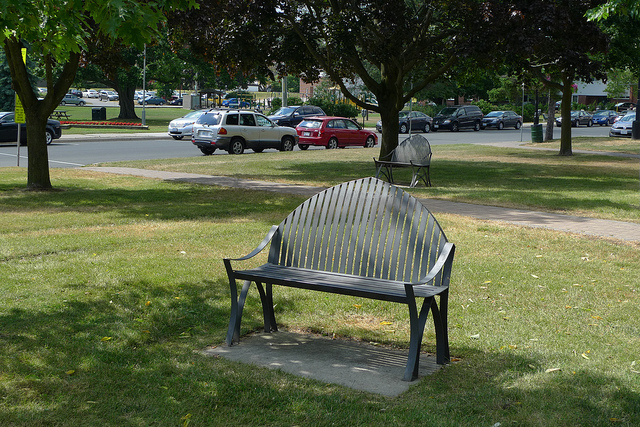
\includegraphics[width=0.68\textwidth]{image/demo.jpg}
    \caption{示例图片}
  \end{figure}
\end{frame}

%%%%%%%%%%%%%%%%%%%%%%%%%%%%%%%%%%%%%%%%%%%%%%%%%%%%%%%%%%
% 插入公式推导页
%%%%%%%%%%%%%%%%%%%%%%%%%%%%%%%%%%%%%%%%%%%%%%%%%%%%%%%%%%
\begin{frame}{Annual Performance Metrics}
  Key Equation Analysis

  \vspace{1em}

  \begin{center}
    \BehindEqBox{
      $\displaystyle
      S = \underbrace{\sum_{i=1}^{N} \textcolor{myorange}{w_i}\, \textcolor{mygreen}{s_i}}_{\textcolor{midblue}{\textbf{Core Score}}} \;+\;
      \overbrace{\left( {\frac{1}{N} \sum_{j=1}^{M} \textcolor{myred}{\delta_j}} \right)}^{\textcolor{mypurple}{\textbf{Adjustment Factor}}}
      $
    }
  \end{center}

  \vspace{1em}

  % 解释公式变量
  \[
    \left\{
    \begin{aligned}
      \textcolor{mygreen}{s_i} &\;=\; \text{Standardized score for module } i, \\
      \textcolor{myorange}{w_i} &\;=\; \text{Weight assigned to module } i, \\
      \textcolor{myred}{\delta_j} &\;=\; \text{External adjustment from factor } j.
    \end{aligned}
    \right.
  \]

  \vspace{1em}

  \textbf{Remark:} Here, \(S\) represents the overall performance metric of an annual study. The \textcolor{midblue}{Core Score} is the weighted sum of standardized scores \(s_i\), while the \textcolor{mypurple}{Adjustment Factor} accounts for external influences aggregated via \(\delta_j\).

\end{frame}


% 另一种配置说明 %%%%%%%%%%%%%%%%%%%%%%%%%%%%%%%%%%%%%%%%%%%%%

\begin{frame}{Modified Example}
  \textbf{Usage Example:} Configuration: Background color = \texttt{mypurple}, border=1pt, dashed border.
  \vspace{1em}

%dotted

  \begin{center}
    \BehindEqBox[color=mypurple, style=dashed, border=1pt]{$\displaystyle \int_{0}^{1} x^2\,dx = \frac{1}{3}$}
  \end{center}

  \vspace{1em}

  % 其他公式或内容
  \textbf{Remark:} The formula calculates the definite integral of \(x^2\) over the interval \([0,1]\), representing the area under the curve.
\end{frame}

%%%%%%%%%%%%%%%%%%%%%%%%%%%%%%%%%%%%%%%%%%%%%%%%%%%%%%%%%%
%文字强调块
%%%%%%%%%%%%%%%%%%%%%%%%%%%%%%%%%%%%%%%%%%%%%%%%%%%%%%%%%%
\begin{frame}{Types of Text Emphasis}
In this slide, key concepts will be \alert{emphasized} because they are crucial.  
Please use sparingly to maintain clarity.

\vspace{0.5em}
\begin{block}{Information Block}
This is a general informational block.
\end{block}

\vspace{0.5em}
\begin{alertblock}{Warning}
This is important information inside a red alert block.
\end{alertblock}

\vspace{0.5em}
\begin{exampleblock}{Key Takeaways}
This block highlights essential information in a green box.  
The title of the block is "Key Takeaways".  
Here's an additional line for checking vertical spacing consistency.
\end{exampleblock}

\end{frame}

%%%%%%%%%%%%%%%%%%%%%%%%%%%%%%%%%%%%%%%%%%%%%%%%%%%%%%%%%%
%图表
%%%%%%%%%%%%%%%%%%%%%%%%%%%%%%%%%%%%%%%%%%%%%%%%%%%%%%%%%%
\begin{frame}{Bar charts}

\begin{center}
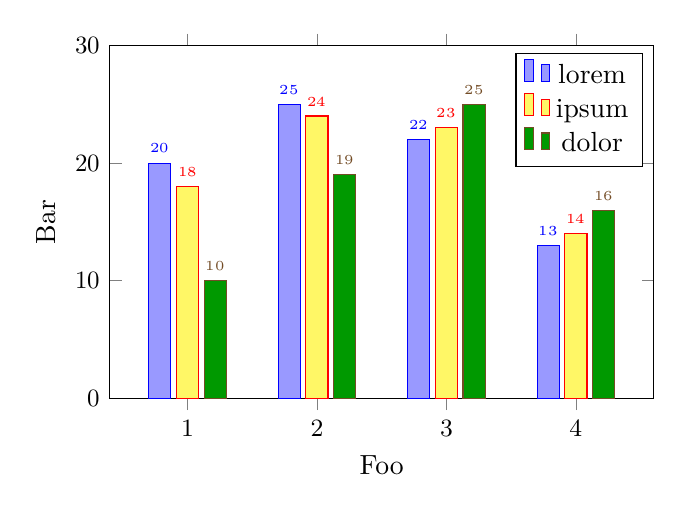
\begin{tikzpicture}
\begin{axis}[
    ybar,
    bar width=8pt,
    width=0.7\textwidth,
    height=0.5\textwidth,
    enlarge x limits=0.2,
    ylabel={Bar},
    xlabel={Foo},
    symbolic x coords={1,2,3,4},
    xtick=data,
    ymin=0,
    ymax=30,
    legend style={at={(0.98,0.98)}, anchor=north east},
    nodes near coords,
    nodes near coords align={vertical},
    every node near coord/.append style={font=\tiny},
    tick label style={font=\small},
]
\addplot+[style={fill=blue!40}] coordinates {(1,20) (2,25) (3,22) (4,13)};
\addplot+[style={fill=yellow!60!white}] coordinates {(1,18) (2,24) (3,23) (4,14)};
\addplot+[style={fill=green!60!black}] coordinates {(1,10) (2,19) (3,25) (4,16)};
\legend{lorem, ipsum, dolor}
\end{axis}
\end{tikzpicture}
\end{center}

\end{frame}

% 问答页
\begin{frame}{Questions and Answers}
  \centering
  \vspace{0.8cm}
  {\Huge \bfseries Q\&A}
\end{frame}

%结束页
\begin{frame}[plain]
  \begin{tikzpicture}[remember picture,overlay]
    % 背景设置:使用深蓝色半透明背景
    \node[fill=midblue, opacity=1, minimum width=\paperwidth, minimum height=\paperheight] at (current page.center) {};
    % THANKS 文本设置:白色大字号
    \node[font=\fontsize{40}{70}\selectfont\bfseries, text=white] at (current page.center) {THANKS};
  \end{tikzpicture}
\end{frame}

\end{document}
